% --------------------------------------------------------------
% This is all preamble stuff that you don't have to worry about.
% Head down to where it says "Start here"
% --------------------------------------------------------------

\documentclass[12pt]{article}

\usepackage[margin=1in]{geometry}
\usepackage{amsmath,amsthm,amssymb}
\usepackage{pgf}
\usepackage{tikz}
\usetikzlibrary{arrows,automata}
\usepackage[latin1]{inputenc}
\usepackage{verbatim}

\newcommand{\N}{\mathbb{N}}
\newcommand{\Z}{\mathbb{Z}}

\newenvironment{theorem}[2][Theorem]{\begin{trivlist}
\item[\hskip \labelsep {\bfseries #1}\hskip \labelsep {\bfseries #2.}]}{\end{trivlist}}
\newenvironment{lemma}[2][Lemma]{\begin{trivlist}
\item[\hskip \labelsep {\bfseries #1}\hskip \labelsep {\bfseries #2.}]}{\end{trivlist}}
\newenvironment{exercise}[2][Exercise]{\begin{trivlist}
\item[\hskip \labelsep {\bfseries #1}\hskip \labelsep {\bfseries #2.}]}{\end{trivlist}}
\newenvironment{problem}[2][Problem]{\begin{trivlist}
\item[\hskip \labelsep {\bfseries #1}\hskip \labelsep {\bfseries #2.}]}{\end{trivlist}}
\newenvironment{question}[2][Question]{\begin{trivlist}
\item[\hskip \labelsep {\bfseries #1}\hskip \labelsep {\bfseries #2.}]}{\end{trivlist}}
\newenvironment{corollary}[2][Corollary]{\begin{trivlist}
\item[\hskip \labelsep {\bfseries #1}\hskip \labelsep {\bfseries #2.}]}{\end{trivlist}}

\begin{document}

% --------------------------------------------------------------
%                         Start here
% --------------------------------------------------------------

\title{Homework 1}%replace X with the appropriate number
\author{Erich Menge\\ %replace with your name
CSCI 4011 - Formal Languages and Automata Theory} %if necessary, replace with your course title

\maketitle

\begin{problem}{1}
Solve this problem with Induction \\
\subsection*{Basis Step}
\begin{align*}
{C(1)} &= \frac{1}{4} \cdot ({(1)^4} + 2 \cdot {(1)^3} + {(1)^2}) = 1\\
{1^3} &= 1\surd
\end{align*}
\subsection*{Inductive Step}
\begin{align*}
{1^3} + {2^3} + ... + {k^3} + {(k + 1)^3} &= \frac{1}{4}({(k + 1)^4} + 2{(k + 1)^3} + {(k + 1)^2})\\
\frac{1}{4}{\rm{(}}{{\rm{k}}^4}{\rm{  +  2}}{{\rm{k}}^3}{\rm{  +  }}{{\rm{k}}^2}{\rm{)  +  (k  +  1}}{{\rm{)}}^3} &= \frac{1}{4}({(k + 1)^4} + 2{(k + 1)^3} + {(k + 1)^2})\\
& = \frac{1}{4}({k^4} + 4{k^3} + 6{k^2} + 4k + 1 + 2{k^3} + 6{k^2} + 6k + 2 + {k^2} + 2k + 1)\\
& = \frac{1}{4}({k^4} + 2{k^3} + {k^2}) + \frac{1}{4}(4{k^3} + 6{k^2} + 6{k^2} + 4k + 6k + 2k + 1 + 2 + 1)\\
& = \frac{1}{4}({k^4} + 2{k^3} + {k^2}) + \frac{1}{4}(4{k^3} + 12{k^2} + 12k + 4)\\
& = \frac{1}{4}({k^4} + 2{k^3} + {k^2}) + {k^3} + 3{k^2} + 3k + 1\\
& = \frac{1}{4}({k^4} + 2{k^3} + {k^2}) + {(k + 1)^3}
\end{align*}
\hfill Q.E.D
\end{problem}
 \newpage
\begin{problem}{2} Part c of Exercise 1.4
\indent \(\{ w|\text{w has an even number of a's and one or two b's}\} \) \\

${A}$ = \(\{ w|\text{w has an even number of a's}\} \)

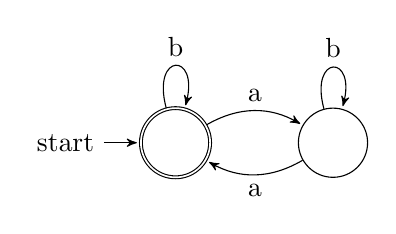
\begin{tikzpicture}[>=stealth',shorten >=1pt,auto,node distance=2cm]
  \node[initial,state,accepting] (S)      {};
  \node[state]         (q1) [right of=S]  {};
 \path[->]
  (S)
    edge [loop above] node{b}(S)
    edge [bend left]node{a}(q1)
  (q1)
    edge [loop above] node{b}(q1)
    edge [bend left]node{a}(S);

\end{tikzpicture} \\

${B}$ = \(\{ w|\text{w has one or two b's}\} \)

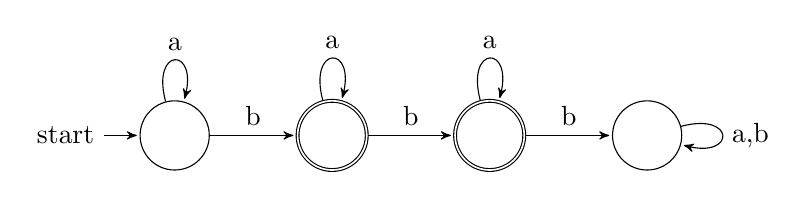
\begin{tikzpicture}[>=stealth',shorten >=1pt,auto,node distance=2cm]
  \node[initial,state] (S)      {};
  \node[state, accepting]         (q1) [right of=S]  {};
  \node[state, accepting]         (q2) [right of=q1]  {};
  \node[state]                    (q3) [right of=q2] {};
  \path[->]
    (S)
      edge [loop above] node{a}(S)
      edge              node{b}(q1)
    (q1)
      edge [loop above] node{a}(q1)
      edge node{b}(q2)
    (q2)
      edge [loop above] node{a}(q2)
      edge node{b}(q3)
    (q3)
      edge [loop right] node{a,b}(q3)
  ;
\end{tikzpicture} \\

${A \times B}$

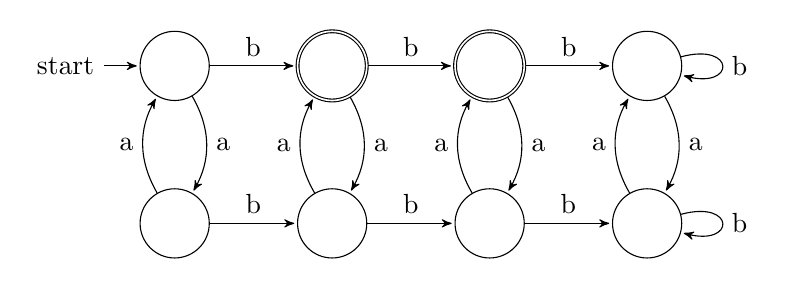
\begin{tikzpicture}[>=stealth',shorten >=1pt,auto,node distance=2cm]
  \node[initial, state] (a1b1) {};
  \node[state, accepting]  (a1b2) [right of=a1b1] {};
  \node[state, accepting]  (a1b3) [right of=a1b2] {};
  \node[state]          (a1b4) [right of=a1b3] {};

  \node[state] (a2b1) [below of=a1b1] {};
  \node[state] (a2b2) [right of=a2b1] {};
  \node[state] (a2b3) [right of=a2b2] {};
  \node[state] (a2b4) [right of=a2b3] {};

  \path[->]
    (a1b1)
      edge node{b}(a1b2)
      edge [bend left] node{a}(a2b1)
    (a1b2)
      edge node{b}(a1b3)
      edge [bend left] node{a}(a2b2)
    (a1b3)
      edge node{b}(a1b4)
      edge [bend left] node{a}(a2b3)
    (a1b4)
      edge [loop right] node{b}(a1b4)
      edge [bend left] node{a}(a2b4)

    (a2b1)
      edge node{b}(a2b2)
      edge [bend left] node{a}(a1b1)
    (a2b2)
      edge node{b}(a2b3)
      edge [bend left] node{a}(a1b2)
    (a2b3)
      edge node{b}(a2b4)
      edge [bend left] node{a}(a1b3)
    (a2b4)
      edge [loop right] node{b}(a2b4)
      edge [bend left] node{a}(a1b4)
  ;
\end{tikzpicture} \\
\end{problem}

\begin{problem}{3} Exercise 1.12
\begin{figure}[h!]
  \centering
  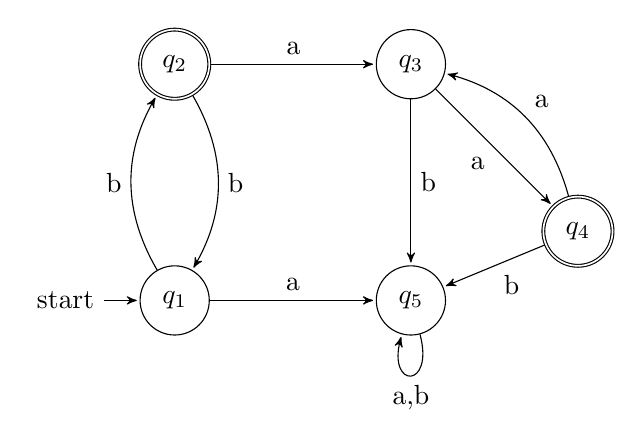
\begin{tikzpicture}[>=stealth',shorten >=1pt,auto,node distance=3cm]
    \node[initial, state] (q1){$q_1$};
    \node[state, accepting] [above of=q1](q2){$q_2$};
    \node[state] [right of=q2](q3){$q_3$};
    \node[state, accepting] [below right of=q3](q4){$q_4$};
    \node[state] [right of=q1](q5){$q_5$};

    \path[->]
      (q1)
        edge node{a}(q5)
        edge [bend left] node{b}(q2)
      (q2)
        edge node{a}(q3)
        edge [bend left] node{b}(q1)
      (q3)
        edge node[swap]{a}(q4)
        edge node {b}(q5)
      (q4)
        edge [bend right] node[swap]{a}(q3)
        edge node {b}(q5)
      (q5)
        edge [loop below] node{a,b}(q5)
    ;
  \end{tikzpicture}
\end{figure}
\end{problem}
 \newpage
\begin{problem}{4}\ \\
\indent $A_1 = \{w|\ w\ \text{contains an even number of 0's\}}$ \\
\indent $A_2 = \{w|\ w\ \text{contains exactly two 1s\}}$ \\

$A_1$: \\
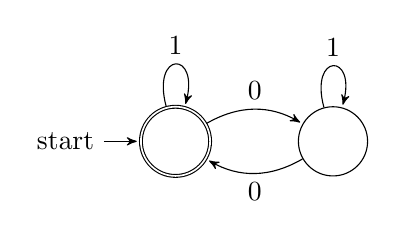
\begin{tikzpicture}[>=stealth',shorten >=1pt,auto,node distance=2cm]
  \node[initial,state, accepting] (S)      {};
  \node[state]         (q1) [right of=S]  {};
  \path[->]
    (S)
      edge [bend left]  node{0}(q1)
      edge [loop above] node{1}(S)
    (q1)
      edge [bend left]  node{0}(S)
      edge [loop above] node{1}(q1)
  ;
\end{tikzpicture} \\

$A_2$: \\
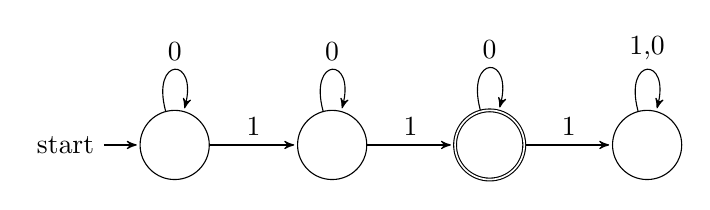
\begin{tikzpicture}[>=stealth',shorten >=1pt,auto,node distance=2cm]
  \node[initial,state] (q1)      {};
  \node[state]         (q2) [right of=q1]  {};
  \node[state, accepting]         (q3) [right of=q2]  {};
  \node[state]         (q4) [right of=q3]  {};
  \path[->]
    (q1)
      edge node{1}(q2)
      edge [loop above] node{0}(q1)
    (q2)
      edge [loop above] node{0}(q2)
      edge node{1}(q3)
    (q3)
      edge [loop above] node{0}(q3)
      edge node{1}(q4)
    (q4)
      edge [loop above] node{1,0}(q4)
  ;
\end{tikzpicture} \\
Let $N_1 =$ ($Q_1$, $\Sigma$, $\delta_1$, $r_1$, $F_1$) recognize $A_1$ \\
Let $N_2 =$ ($Q_2$, $\Sigma$, $\delta_2$, $s_1$, $F_2$) recognize $A_2$ \\
Let $N =$ ($Q$, $\Sigma$, $\delta$, $q_0$, $F$) recognize $N_1 \cup N_2$ \\

\noindent $Q = \{q_0\} \cup Q_1 \cup Q_2 = \{ q_0, r_1, r_2, s_1, s_2, s_3, s_4 \}$ \\
$F = F_1 \cup F_2 = \{ r_1, s_3 \}$ \\

\noindent $
  \delta(q,a) =
  \begin{cases}
    \delta_1(q,a) & q \in Q_1 \\
    \delta_2(q,a) & q \in Q_2 \\
    \{ r_1, s_1 \} & q = q_0 \text{ and } a = \epsilon \\
    \emptyset & q = q_0 \text{ and } a \ne \epsilon
  \end{cases}
$
\begin{figure}[h!]
  \centering
  \caption{Machine N}
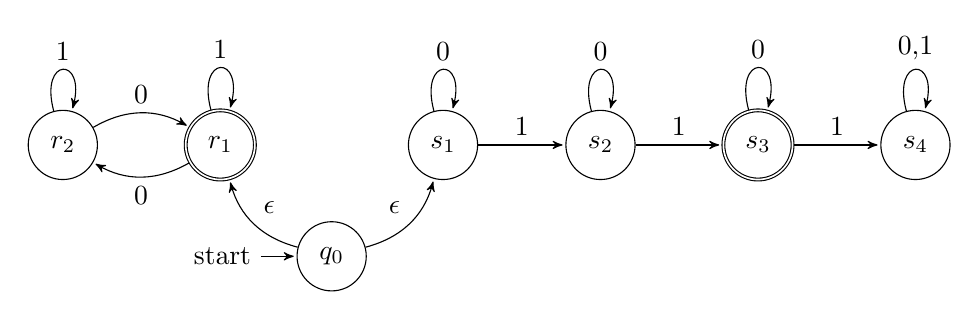
\begin{tikzpicture}[>=stealth',shorten >=1pt,auto,node distance=2cm]
  \node[initial, state] (q0){$q_0$};
  \node[state, accepting] [above left of=q0] (r1){$r_1$};
  \node[state] [left of=r1] (r2){$r_2$};

  \node[state] [above right of=q0] (s1){$s_1$};
  \node[state] [right of=s1] (s2){$s_2$};
  \node[state, accepting] [right of=s2] (s3){$s_3$};
  \node[state] [right of=s3] (s4){$s_4$};
  \path[->]
  (q0)
    edge [bend right]node{$\epsilon$}(s1)
    edge [bend left] node [swap] {$\epsilon$}(r1)
  (r1)
    edge [bend left] node{0}(r2)
    edge [loop above] node{1}(r1)
  (r2)
    edge [bend left] node{0}(r1)
    edge [loop above] node{1}(r2)

  (s1)
    edge [loop above] node{0}(s1)
    edge node{1}(s2)
  (s2)
    edge [loop above] node{0}(s2)
    edge node{1}(s3)
  (s3)
    edge [loop above] node{0}(s3)
    edge node{1}(s4)
  (s4)
    edge [loop above] node{0,1}(s4)
  ;
\end{tikzpicture}
\end{figure}
\end{problem}
 \newpage
\begin{problem}{5}\ \\
  Start the construction by tracing the NFA, recording only reachable steps.

  \noindent
  \ \\
  \begin{minipage}[b]{0.25\linewidth}
    $A = \{ q_0, r_1, s_1 \}$
    \hrule
    $\delta(A,0) = \{ r_2, s_1 \} $ B \\
    $\delta(A,1) = \{ r_1, s_2 \} $ C
  \end{minipage}
  \begin{minipage}[b]{0.25\linewidth}
    $B = \{ r_1, s_2 \}$
    \hrule
    $\delta(B,0) = \{ r_2, s_2 \}$ D \\
    $\delta(B,1) = \{ r_1, s_3 \}$ E
  \end{minipage}
  \begin{minipage}[b]{0.25\linewidth}
    $C = \{ r_2, s_1 \}$
    \hrule
    $\delta(C,0) = \{ r_1, s_1 \}$ F \\
    $\delta(C,1) = \{ r_2, s_2 \}$ D
  \end{minipage}
  \begin{minipage}[b]{0.25\linewidth}
    $D = \{ r_2, s_2 \}$
    \hrule
    $\delta(D,0) = \{ r_1, s_2 \}$ B \\
    $\delta(D,1) = \{ r_2, s_3 \}$ G
  \end{minipage}
  \ \\
  \begin{minipage}[b]{0.25\linewidth}
    $E = \{ r_1, s_3 \}$
    \hrule
    $\delta(E,0) = \{ r_2, s_3 \}$ G \\
    $\delta(E,1) = \{ r_1, s_4 \}$ H
  \end{minipage}
  \begin{minipage}[b]{0.25\linewidth}
    $F = \{ r_1, s_1 \}$
    \hrule
    $\delta(F,0) = \{ r_2, s_1 \}$ C \\
    $\delta(F,1) = \{ r_1, s_2 \}$ B
  \end{minipage}
  \begin{minipage}[b]{0.25\linewidth}
    $G = \{ r_2, s_3 \}$
    \hrule
    $\delta(G,0) = \{ r_1, s_3 \}$ G \\
    $\delta(G,1) = \{ r_2, s_4 \}$ I
  \end{minipage}
  \begin{minipage}[b]{0.25\linewidth}
    $H = \{ r_1, s_4 \}$
    \hrule
    $\delta(H,0) = \{ r_2, s_4 \}$ I \\
    $\delta(H,1) = \{ r_1, s_4 \}$ H
  \end{minipage}
  \ \\
  \begin{minipage}[b]{0.25\linewidth}
    $I = \{ r_1, s_4 \}$
    \hrule
    $\delta(I,0) = \{ r_2, s_4 \}$ I \\
    $\delta(I,1) = \{ r_1, s_4 \}$ I
  \end{minipage}

  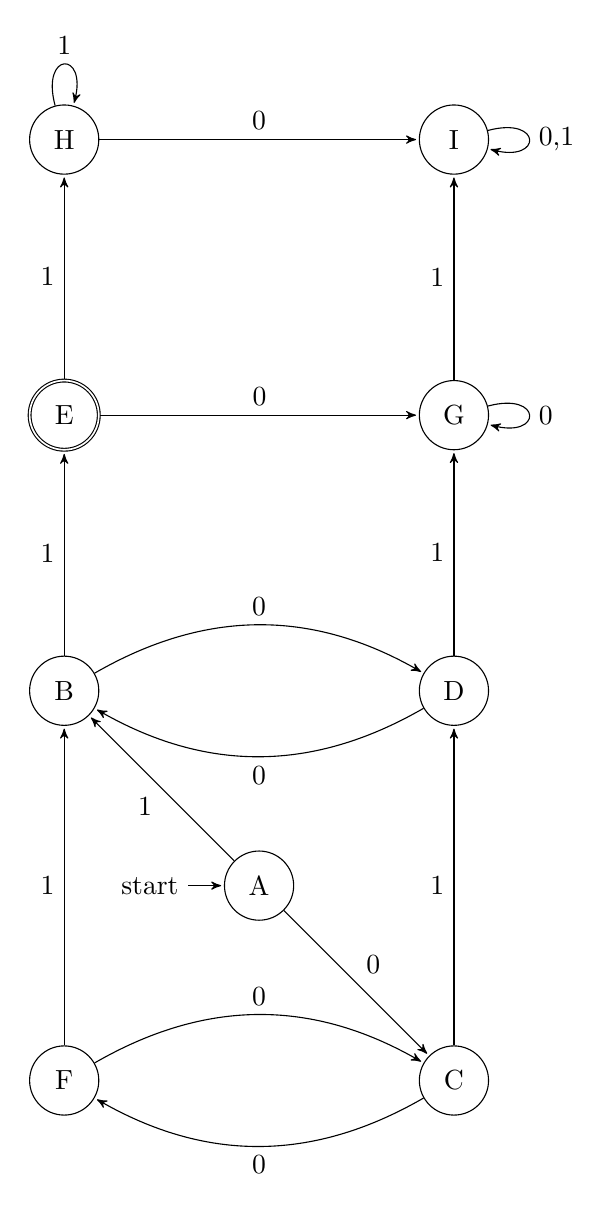
\begin{tikzpicture}[>=stealth',shorten >=1pt,auto,node distance=3.5cm]
    \node[initial, state]                 (A){A};
    \node[state] [above left of=A]        (B){B};
    \node[state] [below right of=A]       (C){C};
    \node[state] [above right of=A]       (D){D};
    \node[state, accepting] [above of=B]  (E){E};
    \node[state] [below left of=A]        (F){F};
    \node[state] [above of=D]             (G){G};
    \node[state] [above of=E]             (H){H};
    \node[state] [above of=G]             (I){I};

    \path[->]
      (A)
        edge node{1}(B)
        edge node{0}(C)
      (B)
        edge [bend left]node{0}(D)
        edge node{1}(E)
      (C)
        edge [bend left]node{0}(F)
        edge node{1}(D)
      (D)
        edge node{1}(G)
        edge [bend left]node{0}(B)
      (E)
        edge node{1}(H)
        edge node{0}(G)
      (F)
        edge [bend left]node{0}(C)
        edge node{1}(B)
      (G)
        edge [loop right] node{0}(G)
        edge node{1}(I)
      (H)
        edge node{0}(I)
        edge [loop above] node{1}(H)
      (I)
        edge [loop right] node{0,1}(I)
    ;
  \end{tikzpicture}
\end{problem}


\begin{problem}{6} Exercise 1.25 from the book. \\

\noindent Let an FST defined by 5-tuple $(Q, \sigma, \delta, $q_0$, \tau)$ recognize language $w$ where: \\
Q is the set of states. \\
$\sigma$ is the alphabet \\
$\delta: Q \times \sigma \rightarrow \tau$ \\
$q_0 \in Q$ is the start state. \\
and $\tau$ represents the set of possible outputs. \\

\noindent{\bf Computation:} \\

\noindent Let $M = A FST$ and let $w = w_1w_2 \ldots w_n$ be a string where $w_i$ is a member of $\sigma$.
Then $M$ produces $\tau$ from $w$ if a sequence of states $r_0,r_1 \ldots r_n$ in Q exists, and if:
\begin{enumerate}
\item $r_0 = q_0$
\item $\delta(r_i, w_i + 1) = r_i + 1$ for $i = 0 \ldots n - 1$
\item $r_1 \ldots r_n \in \tau$
\end{enumerate}

\end{problem}

\begin{problem}{7} Exercise 1.31 from the book. \\

\noindent A language is regular if it is recognized by some finite automaton. \\

\noindent So for $A$ we have some NFA with $(Q, \Sigma, \delta, q_0, F)$. \\

\noindent We define $A^R$ to be another NFA with 5-tuple $(Q', \Sigma, \delta', q_0', F')$ where: \\
$Q' = Q$. \\
$\delta'$ is $\delta$ with all transitions reversed. \\
$F'$ is the set of start states of $A$. \\
$q_0'$ is the set of accept states of $A$. \\

\noindent Then the new NFA works the same as the first NFA, only in reverse. \\

\noindent This proves $A^R$ is regular by construction. \\

\end{problem}

\begin{problem}{8} Do Exercise 1.32 from the book. \\
\end{problem}


% --------------------------------------------------------------
%     You don't have to mess with anything below this line.
% --------------------------------------------------------------

\end{document}